% Options for packages loaded elsewhere
\PassOptionsToPackage{unicode}{hyperref}
\PassOptionsToPackage{hyphens}{url}
%
\documentclass[
  12pt,
]{article}
\usepackage{lmodern}
\usepackage{setspace}
\usepackage{amsmath}
\usepackage{ifxetex,ifluatex}
\ifnum 0\ifxetex 1\fi\ifluatex 1\fi=0 % if pdftex
  \usepackage[T1]{fontenc}
  \usepackage[utf8]{inputenc}
  \usepackage{textcomp} % provide euro and other symbols
  \usepackage{amssymb}
\else % if luatex or xetex
  \usepackage{unicode-math}
  \defaultfontfeatures{Scale=MatchLowercase}
  \defaultfontfeatures[\rmfamily]{Ligatures=TeX,Scale=1}
\fi
% Use upquote if available, for straight quotes in verbatim environments
\IfFileExists{upquote.sty}{\usepackage{upquote}}{}
\IfFileExists{microtype.sty}{% use microtype if available
  \usepackage[]{microtype}
  \UseMicrotypeSet[protrusion]{basicmath} % disable protrusion for tt fonts
}{}
\makeatletter
\@ifundefined{KOMAClassName}{% if non-KOMA class
  \IfFileExists{parskip.sty}{%
    \usepackage{parskip}
  }{% else
    \setlength{\parindent}{0pt}
    \setlength{\parskip}{6pt plus 2pt minus 1pt}}
}{% if KOMA class
  \KOMAoptions{parskip=half}}
\makeatother
\usepackage{xcolor}
\IfFileExists{xurl.sty}{\usepackage{xurl}}{} % add URL line breaks if available
\IfFileExists{bookmark.sty}{\usepackage{bookmark}}{\usepackage{hyperref}}
\hypersetup{
  hidelinks,
  pdfcreator={LaTeX via pandoc}}
\urlstyle{same} % disable monospaced font for URLs
\usepackage[margin=1in]{geometry}
\usepackage{longtable,booktabs}
\usepackage{calc} % for calculating minipage widths
% Correct order of tables after \paragraph or \subparagraph
\usepackage{etoolbox}
\makeatletter
\patchcmd\longtable{\par}{\if@noskipsec\mbox{}\fi\par}{}{}
\makeatother
% Allow footnotes in longtable head/foot
\IfFileExists{footnotehyper.sty}{\usepackage{footnotehyper}}{\usepackage{footnote}}
\makesavenoteenv{longtable}
\usepackage{graphicx}
\makeatletter
\def\maxwidth{\ifdim\Gin@nat@width>\linewidth\linewidth\else\Gin@nat@width\fi}
\def\maxheight{\ifdim\Gin@nat@height>\textheight\textheight\else\Gin@nat@height\fi}
\makeatother
% Scale images if necessary, so that they will not overflow the page
% margins by default, and it is still possible to overwrite the defaults
% using explicit options in \includegraphics[width, height, ...]{}
\setkeys{Gin}{width=\maxwidth,height=\maxheight,keepaspectratio}
% Set default figure placement to htbp
\makeatletter
\def\fps@figure{htbp}
\makeatother
\setlength{\emergencystretch}{3em} % prevent overfull lines
\providecommand{\tightlist}{%
  \setlength{\itemsep}{0pt}\setlength{\parskip}{0pt}}
\setcounter{secnumdepth}{5}
\usepackage{etoolbox}
\usepackage{fancyhdr}
\usepackage{lipsum}
\patchcmd{\maketitle}{\end{titlepage}}{\thispagestyle{titlepagestyle}\end{titlepage}}{}{}
\fancypagestyle{titlepagestyle}{\fancyhf{}\fancyfoot[C]{\emph{This text needs to appear on the title page}}\renewcommand{\headrulewidth}{0 mm}}
\usepackage{xcolor}
\usepackage[format=plain,font=it]{caption}
\usepackage{floatrow}
\floatsetup[figure]{capposition=top}
\floatsetup[table]{capposition=top}
\usepackage[small]{titlesec}
\usepackage{titlesec}
\titleformat*{\section}{\large\bfseries}
\titlespacing{\section}{0pt}{12pt}{-5pt}
\titleformat*{\subsection}{\normalsize\itshape}
\titlespacing{\subsection}{0pt}{6pt}{-5pt}
\titlelabel{\thetitle.\hspace{0.2cm}}
\raggedright
\usepackage{rotating}
\newcommand{\beginappendix}{\setcounter{table}{0}  \renewcommand{\thetable}{A\arabic{table}} \setcounter{figure}{0} \renewcommand{\thefigure}{A\arabic{figure}}}
\usepackage{helvet}
\renewcommand{\familydefault}{\sfdefault}
\usepackage{booktabs}
\usepackage{longtable}
\usepackage{array}
\usepackage{multirow}
\usepackage{wrapfig}
\usepackage{float}
\usepackage{colortbl}
\usepackage{pdflscape}
\usepackage{tabu}
\usepackage{threeparttable}
\usepackage{threeparttablex}
\usepackage[normalem]{ulem}
\usepackage{makecell}
\usepackage{xcolor}
\ifluatex
  \usepackage{selnolig}  % disable illegal ligatures
\fi

\author{}
\date{\vspace{-2.5em}}

\begin{document}

\begin{titlepage}
\begin{center}
\vspace*{5cm}
\LARGE
\textbf{The Effect of Distrust on Government Stringency During the Covid-19 Pandemic}


\vspace{1.5cm}
\large
Candidate Number: KFHH0

\vspace{0.5cm}
Word Count: 8282

\vfill

Dissertation submitted in part-fulfilment of the Masters Course in Public Policy, UCL,  September 2021.

% \afterpage{\blankpage}
\end{center}
\end{titlepage}

\begin{center}
\textbf{Acknowledgements}

To my supervisor, Prof. Ben Lauderdale for his support and advice.

To my darling Annabelle for putting up with my ramblings about distrust.

To my parents for their constant support.
\pagenumbering{gobble} 
\end{center}

\pagebreak

\begin{center}
\vspace*{5cm}
\textbf{Abstract}
\end{center}
Since Covid-19 spread across the world, governments have sought to control it through imposing strict restrictions on their citizens, from work-place closures to stay at home orders and curfews. But the stringency of these responses has varied across countries, with some like Belarus having very few restrictions and others, like New Zealand, having incredibly strict responses. This paper explains these differences in response by treating the pandemic as a collective action problem and arguing that distrust in other people has played an important role in how countries attempt to solve this collective action problem, with higher levels of distrust creating a demand for intervention from the government. By using a random effects regression analysis, this paper finds that higher levels of distrust leads to higher levels of stringency during the pandemic. Further analysis finds that this effect has changed over the course of the pandemic, with a stronger effect as the pandemic has gone on.
\pagenumbering{gobble} 
\pagebreak

\setstretch{2}
\pagenumbering{gobble} 
\clearpage
\tableofcontents
\pagenumbering{gobble} 
\newpage
\pagenumbering{arabic}

\hypertarget{introduction}{%
\section{Introduction}\label{introduction}}

In December 2019 the first cases of a novel coronavirus were detected in the Wuhan province of China. The virus quickly spread around the world and the World Health Organisation (WHO) declared a global pandemic in March 2020 (Cucinotta \& Vanelli, 2020). At this time treatments were in the very early stages of research and no vaccine had been developed (GlobeNewswire, 2020). This left governments struggling to control its spread. Many chose to impose strict lockdowns on their citizens -- curtailing freedoms in an attempt to slow the spread and avoid hospitals from being overrun. But the stringency of restrictions has varied greatly from country to country, with many governments imposing social-distancing measures such as stay-at-home orders and workplace closures, while other countries opted not to implement these policies or implemented them to a lesser degree (Hale, et al., 2021). By treating the Covid-19 pandemic as a large-scale collective action problem, this paper attempts to explain these differences in the stringency of government restrictions as a causal effect of a country's level of distrust.\\
~\\
By trust and distrust, this paper refers to an individual's trust or lack of trust in other people, which is aggregated to the country level. A more detailed account of how this type of trust is measured is given in the data section, but it is important to note that interpersonal trust is distinct from trust in the government. It is interpersonal trust that plays an important role in solving collective action problems. Elinor Ostrom, one of the most influential proponents of collective action theory, has shown that when a group's level of trust is higher, they are more likely to achieve collective action without enforcement or intervention by a third party (Ostrom, 2009). But when individuals do not trust that others will take steps to achieve collective action, they are likely to turn to the government to intervene (Harring, et al., 2021). This leads to the hypothesis that countries with higher levels of distrust will be more likely to have higher levels of government stringency during the pandemic, where government stringency is the strictness of lockdown style restrictions imposed by a government.\\
~\\
To test the hypothesis, this paper uses a random effects model, which allows for the estimation of the effect that a country's pre-pandemic level of distrust has on the level of government stringency during the pandemic. The results of the analysis provide strong evidence in support of the hypothesis, finding that, when controlling for a wide variety of potentially confounding variables, higher levels of distrust cause higher levels of government stringency.\\
~\\
The next section in this paper will give an overview of the literature on how trust affects different outcome measures, how this relates to collective action theory and research that has been conducted on trust and Covid-19 outcomes. The third section will outline the research design, showing how a random effects model can estimate the effect of distrust and why it is preferred over other methods, as well as outlining what data is used in the model and why these variables should be included. The fourth section will present the results of the analysis along with a discussion of these results. The fifth section will explain the limitations of this research and the assumptions upon which the results rest. Finally, the paper will finish with some concluding remarks, implications for collective action theory and recommendations for future research.\\

\hypertarget{literature-review-and-theory}{%
\section{Literature Review and Theory}\label{literature-review-and-theory}}

\hypertarget{the-role-of-trust-in-society}{%
\subsection{The role of trust in society}\label{the-role-of-trust-in-society}}

A lot of research on the effect of trust comes under the broader category of social capital. Social capital can be thought of as the resources that fuel relationships and cooperation between people (Häuberer, 2011), made up of ``social networks, cooperative norms and interpersonal trust'' (Knack, 2002, p.~772). Knack (2002) argues that the popularity of using measures of social capital in research has led the use of `overly-aggregated' indices, making it difficult to identify the precise mechanisms at play. As such, this paper will follow in Knack's effort of disaggregating social capital by focusing on just the effect of interpersonal trust.\\
~\\
Interpersonal trust has been shown to be an important causal factor to many different societal outcomes. It plays an important role in economic growth (Helliwell \& Putnam, 1995; Zak \& Knack, 2001), which is in part the result of trust having a causal effect on both schooling and law and order (Bjornskov, 2012). Trust has also been shown to have had an effect on support for social welfare programs (Daniele \& Geys, 2015), the financial development of individuals (Guiso, et al., 2004), as well as trade, investments and FDI (Guiso, et al., 2009).\\

\hypertarget{trust-and-collective-action}{%
\subsection{Trust and collective action}\label{trust-and-collective-action}}

The power that interpersonal trust appears to have in society can in part be explained by the role that trust plays in cooperation, which is crucial to solving collective action problems. Collective action occurs when individuals act in the interest of the collective group, and a collective action problem arises when an individual, who acts in their own interest, is not incentivised to act in the collective interest (Ostrom, 2009). The theory originally proposed by Olson (1965) argues that rational individuals seek to maximise their gains and minimise their losses, but often this rational individual is incentivised to act against the collective interest (which also ends up going against their own interests). An example of this is the problem of climate change (Harring, et al., 2021), where it is in the collective interest to take actions to prevent climate change. From the individual's perspective, if they believe that everyone else will take action to prevent climate change, then there is no point in them taking action, as their individual actions will have close to zero additional effect on achieving the collective goals. Likewise, if they believe that no one will act to prevent climate change then there is also no point in taking action, as solving the problem requires everyone to act and one individual's actions will have no real effect on achieving a climate change free world. This leads to a situation where no individuals are incentivised to act to prevent climate change even though it is in the collective interest to do so, therefore resulting in a collective action problem.\\
~\\
Solving a collective action problem requires individuals to be incentivised to act in the collective interest, and for Olson, this is most easily achieved through intervention by the state (Olson, 1982). The state has the power to coerce people into acting collectively, and is most commonly achieved through taxes, fines, and laws which are enforced with the threat or use of force. Without the state, it would not be in the individual interest to pay for roads, as the individual could wait for someone else to pay for roads and freeride at their expense. However, with intervention from the state, if an individual does not pay their taxes for the road then the state can threaten them with imprisonment, providing the individual with incentive to act collectively.\\
~\\
Elinor Ostrom expanded on Olson's collective action theory and proposed that there are many situations in which groups can achieve collective action without intervention from the state. She developed theory and evidence for how different factors affect the chances of achieving collective action, which include the number of participants involved, face-to-face communication between participants, and information about past actions (Ostrom, 2009, p.~189). One factor that plays a crucial role in the likelihood of achieving collective action is interpersonal trust. If an individual trusts that others will act in the collective interest then they are more likely themselves to act collectively, which then further leads to others finding that individual trustworthy, and creates a loop of positive reinforcement (Ostrom, 2009, pp.~201-202).\\

\hypertarget{trust-and-the-covid-19-pandemic}{%
\subsection{Trust and the Covid-19 pandemic}\label{trust-and-the-covid-19-pandemic}}

Collective action theory can also be applied to the Covid-19 pandemic. During the pandemic many individuals have not been incentivised to take action to prevent the spread of the virus -- such as distancing themselves from friends and family. From an individual's perspective, similarly to the climate change problem, whether they socially distance or not will have little to no impact on the spread of the virus. Given the large cost of socially distancing to the experience of `normal life', individuals acting purely in their individual interest are not incentivised to act collectively with regard to the pandemic\footnote{Due to the nature of the pandemic being the spread of a virus, there is additional individual incentive to socially distance for some individuals. People who are more likely to become seriously ill from the virus will have an incentive to reduce contact with other people. However, there are still large parts of the population who do not have this incentive, either because they are not at higher risk of the getting seriously ill from the virus or because they do not believe they are. Therefore, the pandemic can still be considered a collective action problem.}. Harring et al., (2021) label the pandemic as a `large-scale collective action problem' which is characterised by very large numbers of people needing to cooperate in order to achieve collective action. In the case of the pandemic almost the entire global population is required to act collectively to achieve the collective goal of living in a Covid-19 free world. This makes it far less likely to achieve collective action without intervention from a third-party.\\
~\\
As with other collective action problems, trust plays an important role in the likelihood of collective action being achieved, and there have already been a few studies exploring how trust affects different Covid-19 outcomes. It has been shown that higher levels of trust are associated with higher levels of compliance in response to lockdown policies (Bargaina \& Aminjonov, 2020; Goldstein \& Wiedemann, 2021). Another study, by Elgara, et al., (2020), shows evidence that higher levels of trust leads to more deaths during the pandemic, the opposite result that the authors had predicted which appears to go against the theory of collective action. It was expected that more trust would lead to more people acting collectively, which would in turn lead to a lower death toll. The authors' explanation for this result was that higher trusting countries may have stronger group bonds, therefore creating difficulties in social distancing, or because of higher trusting countries are more susceptible to misinformation (Elgara, et al., 2020). However, their paper has also been criticised for problems in methodology, with a potentially inaccurate model specification (Lindström, 2020), and their result should be interpreted with caution. So far, no research has explored the effect of trust on government stringency in response to the pandemic and this paper aims to fill that gap.\\

\hypertarget{hypothesis}{%
\subsection{Hypothesis}\label{hypothesis}}

Large-scale collective action problems already create a demand for intervention by the government, due to them being so hard to solve without intervention (Harring, et al., 2021). It is expected that in countries where there are high levels of distrust in others, individuals will not believe that others will take steps to reduce the spread of Covid-19 and as such are less likely to be able to solve the collective action problem without intervention. This creates demand and support for intervention by the government, which in turn leads to the government meeting this demand with higher levels of policy stringency -- either because there is less opposition to the policies that the government wants to introduce or because the population pressures the government to introduce more stringent policies. This theoretical mechanism leads to the hypothesis that higher levels of distrust in others before the pandemic causes higher levels of government stringency during the pandemic.\\

\hypertarget{research-design-and-data}{%
\section{Research Design and data}\label{research-design-and-data}}

\hypertarget{why-random-effects}{%
\subsection{Why random effects?}\label{why-random-effects}}

The data used in this study is country level time-series panel data, with some variables that are time-invariant (measured once for each country) and others that are time-varying over the course of the pandemic. The problem faced when analysing time-series data using regression analysis is that a standard pooled linear regression assumes the independence of residuals. This is to say that once all confounders are adjusted for, there are no longer any correlations between variables (Bell \& Jones, 2015, p.~135). With time-series country level data, this assumption can rarely be met because the variables measured within a country are highly likely to be dependent on the measure of that same variable in previous years or days. Using a pooled regression for this type of data will lead to a misspecification of the model, with inaccurate estimates and standard errors.\\
~\\
To overcome this problem, this paper will use a random effects (RE) model to test whether distrust causes a more stringent government response to the pandemic\footnote{All statistical models and analysis in this paper are produced with the R programming language (R Core Team, 2020) and random effects models are created with the lme4 package (Bates, et al., 2015). The replication data, analysis scripts and a description of all packages used are available at: https://github.com/KFHH0/dissertation}. This type of model, also called a hierarchical/mixed model, solves the problem of independence in time-series data by partitioning the residual variance into higher- and lower-level variance within units (Bell \& Jones, 2015, p.~135). Lower-level units are units that are nested within higher level units, for example, cities are a lower-level unit nested within the higher-level unit of countries. In the case of this study, time-varying observations (e.g., government stringency) are lower-level observations nested within the higher-level time-invariant observations (e.g., distrust), where the time-varying observations are measured every day during the pandemic and the time-invariant observations were measured once before the pandemic. The RE model not only solves the problem of correlated residuals but allows for the estimation of the effect that a higher-level variable has on a lower-level one (Imai \& Kim, 2019). So, a random effects model makes it possible to measure the effect that distrust (a high-level variable) has on government stringency (a low-level variable).\\
~\\
This method goes beyond the ability of the commonly used fixed effects (FE) model. FE models also solve the problem of correlated residuals, although they do it by adding dummy variables for each high-level entity (in this study there would be a dummy variable for each country). This has the added benefit of controlling for all high-level time-invariant confounding factors, but due to the fact the there is a dummy variable for each high-level entity, an FE model cannot estimate the effect that a high-level variable has on a lower-level variable (Imai \& Kim, 2019). So, for this study, it would not be possible to specify an FE model that can test the hypothesis that distrust has a causal effect on government stringency.\\
~\\
Given that distrust is not randomly assigned to countries, a model estimating its effect is subject to selection bias and, as a result, potentially confounding variables must be adjusted for. In contrast to an FE model, which controls for all potential high-level time-invariant confounding factors, an RE model can be confounded by time-invariant factors. As such high-level time-invariant factors must be controlled for in the RE model. For this study, that means controlling for variables that are associated both with the level of distrust and the level of government stringency.\\

\hypertarget{data-sources}{%
\subsection{Data Sources}\label{data-sources}}

The outcome variable in this study is a measure of government stringency in response to the pandemic. This measure is the stringency index from the Oxford COVID-19 Government Response Tracker (OxCGRT) -- a continuously updated dataset of 19 policy measures which are measured daily (Hale, et al., 2021, p.~529). The stringency index is composed of 9 of the measures which are focused on `lockdown' style policies\footnote{Includes: school closures, workplace closures, cancellation of public events, restrictions on gatherings, public transport closures, public information campaigns, stay at home orders, restrictions on internal movement, and restrictions on international travel.} (Hale, et al., 2021, p.~530). Figure \ref{fig:stringency-plot} shows how the stringency index has changed over the course of the pandemic for the countries included in this study, it shows that in March, when the pandemic was declared by the WHO, the average stringency shot up and then gradually began to fall and level out. It is also split into high and low distrust countries\footnote{A country is considered to have a low level of distrust if it is below the median (78.98) and a high level if it is equal to or above the median.}, showing that countries with higher levels of distrust have persistently had a more stringent response. Figure \ref{fig:stringency-sd} (Figures and tables beginning with `A' are in the appendix) shows how the standard deviation for government stringency has changed throughout the pandemic; variance is highest during periods when levels of stringency are changing -- either during the beginning or end of waves of the pandemic.\\
~\\

\begin{figure}
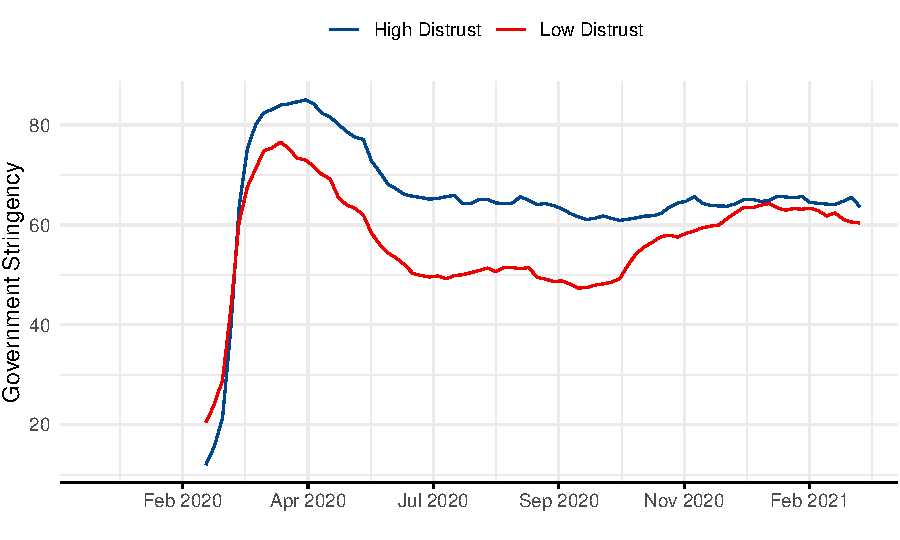
\includegraphics[width=0.8\linewidth]{write_up_test_files/figure-latex/stringency-plot-1} \caption{Government Stringency during the Pandemic}\label{fig:stringency-plot}
\end{figure}

\hfill\break
Table \ref{tab:stats} shows the mean and standard deviation for all of the high-level independent variables. The independent variable of interest is the level of distrust in other people. This variable is based on the measure of trust in the European Values Study/World Values Survey (EVS/WVS, 2021a). The EVS/WVS conducted surveys across 81 countries between 2017 and 2020. Of these countries Canada, Iran, Ethiopia, Singapore, and Zimbabwe had data collected after the pandemic had been declared (EVS/WVS, 2021b, pp.~8-11; Cucinotta \& Vanelli, 2020), as such they are removed from the study to avoid the government stringency in response to the pandemic having a reverse effect on the level of distrust. The question asked to measure trust is: `Generally speaking, would you say that most people can be trusted or that you can't be too careful in dealing with people?' (EVS/WVS, 2021b, p.~121). The distrust variable in this study is the percent of people within a country who in response to this question answered that `you can't be too careful in dealing with people'. As it is measured as a percentage, it varies is on a scale of 0 to 100, with a range of 26.03 (Denmark) to 98.40 (Albania) and a mean of 74.31.\\
~\\

\begin{table}

\caption{\label{tab:stats}Summary statistics for each high-level variable}
\centering
\begin{tabular}[t]{lcc}
\toprule
Variable & Mean (SD) & Missing\\
\midrule
Distrust in People & 74.31 (18.73) & 0\\
Log of GDP per Capita & 9.36 (1.23) & 2\\
GDP Growth & 2.15 (2.97) & 1\\
Education Index & 0.76 (0.14) & 6\\
Log of Conflict Index & 8.11 (1.64) & 6\\
\addlinespace
Confidence in Government & 42 (22.59) & 1\\
Polity & 6.01 (5.5) & 7\\
Population Density (per km2) & 139.85 (182.56) & 3\\
Population over age 65 & 13.28 (6.58) & 2\\
Global Health Security Index & 51.76 (13.03) & 4\\
\addlinespace
Gini Coefficient & 34.35 (6.93) & 17\\
\bottomrule
\multicolumn{3}{l}{\textsuperscript{} \small{SD = Standard Deviation}}\\
\end{tabular}
\end{table}

Confidence in government is another variable from EVS/WVS that is controlled for in the RE model. This variable is measured in the survey by asking how much confidence the participant has in the government, with the options: A great deal, quite a lot, not very much and none at all (EVS/WVS, 2021b, p.~171). The variable included in this study is calculated by taking the percent of respondents within a country who answered either a great deal or quite a lot, making the variable a measure of the percent of population that have confidence in the government. The variable is included in the model because it potentially confounds the relationship between distrust and stringency. Higher levels of confidence in government are associated with lower levels of distrust in other people, as there may be similar reasons for not having trust in people as to not having confidence in the government (such as high levels of crime). Figure \ref{fig:conf-plots} shows this relationship between confidence in government and distrust, and although there is a slight negative correlation between the two variables they are not highly correlate and appear to be distinct in what they are measuring. Confidence in government might also be cause higher levels of government stringency -- if people are less confident in the government they may demand fewer restrictions from it, therefore it is included in the model to adjust for any potential confounding effect.\\
~\\
There are three measures of development that are included in the model. The first two are economic measures: log of GDP per capita and GDP growth (World Bank, 2021a; World Bank, 2021b). The other measure of development is the education index, which is the mean years of schooling for adults and expected years of schooling for children (United Nations Development Programme, 2020). These measures of development are controlled for because higher development is associated with lower levels of distrust and a country's level of development may contribute to differences in priorities for the government during the pandemic. This relationship is shown in figure \ref{fig:gdp-plots} for the association of logged GDP per capita with distrust and government stringency.\\
~\\
Another important variable that needs to be adjusted for is the Global Health Security Index (GHS Index) (Nuclear Threat Initiative, Johns Hopkins Center for Health Security, The Economist Intelligence Unit, 2019). The GHS index is a measure of how prepared a country is for a pandemic, composed of 6 categories of preparedness including robustness of the health system, early detection and reporting of pandemics, and risk environment. GHS index is negatively associated with distrust, as shown in Figure \ref{fig:ghs-plots}. Higher levels of GHS are predictive of lower levels of distrust, which is likely explained by similar reasons as to how development predicts distrust. Although the GHS index has no clear association with government stringency in Figure \ref{fig:ghs-plots} it is still likely to have a causal effect on stringency index and the lack of any clear association is perhaps due it potentially having both a positive and negative effect. It could lead to a more stringent response because these policies have already been planned for, or could lead to a less stringent response because the virus is able to be maintained without strict lockdowns. Either way, it should be controlled for in the analysis.\\
~\\
The level of internal conflict within a country is also adjusted for using the logged conflict index from the `Cross-National Time-Series Data Archive' (CNTS), which is a weighted average of the number of eight different types of internal conflict events: major government crises, terror attacks, riots, assassinations, general strikes, purges, revolutions and anti-government demonstrations (Banks \& Wilson, 2020). These internal conflict events are likely to lead to higher levels of distrust, for instance, the 2005 London terrorist attacks led to an increase in distrust from 56\% to 64\% (Giordano \& Lindstrom, 2016). A country with higher levels of internal conflict is also likely to affect the government response to the pandemic, either as a result of government priorities or because of the culture that the internal conflict leads to. The log of conflict index is taken because a unit increase conflict in countries with high conflict will likely have less of an effect than the same increase in countries with low conflict, figure \ref{fig:conflict-log} shows this association and how taking the log adjusts for it.\\
~\\
Another variable used from the CNTS is population density, measured as population per square kilometre (Banks \& Wilson, 2020). Areas with higher population density are associated with higher levels of distrust (House \& Wolf, 1978), potentially as a result of individuals being in contact with more people that they don't know and are less likely to be inclined to trust. Countries with high population density are also at higher risk of Covid-19 spreading (Bhadra, et al., 2021), in part due to people being in closer proximity, and as such the government's in these countries are likely to be inclined to impose stricter restrictions.\\
~\\
The polity measure from Systemic Peace, which is a measure of regime authority and democracy within a country (Marshall \& Gurr, 2020), is also adjusted for. It is measured on a scale of --10 to 10, where --10 is the most authoritarian a state can be and 10 is the least. Democracy is associated with lower levels of distrust, although it is not clear which direction this association goes in and it is likely the two are interdependent (Warren, 1999). It is also likely to lead to lower levels of stringency due to the rule of law generally being less strict in more democratic and less authoritarian countries. The last high-level measure that is adjusted for is the Gini-coefficient, which is a measure of income inequality, in particular, this study uses the measure of disposable income inequality (Solt, 2020). Inequality within groups has been shown to lead to higher levels of distrust within those groups (Twenge, et al., 2014) and figure \ref{fig:gini-plots} shows that this association appears to hold for countries. It also shows that inequality is associated with higher levels of stringency during the pandemic, although it is not clear what the mechanism is here.\\
~\\
In addition to the high-level variables that are included in the main analysis, two low-level variables are also included in an additional analysis. These variables are time-variant and are measured every day, the first of which is a measure of new deaths per million (Dong, et al., 2020). This variable is the number of confirmed deaths from Covid-19 for each day for each country. Figure \ref{fig:deaths-change} shows how the variable changes over the course of the pandemic. There are some reliability issues with this data; one problem is that limited testing in many countries means the true number of Covid-19 deaths is likely to be higher than those reported (Ritchie, et al., 2020a). Another problem is that both the method of recording deaths and when they are reported varies between countries, and this can make comparisons between countries difficult. That being said, the variable can still be useful in this analysis as it is still associated with both stringency and distrust, as shown in figure \ref{fig:deaths-plots}. However, it is not included in the main model due to both the problems with reliability and also the fact that the variables are determinates of each other\footnote{The previous level of stringency will be a determinate of new deaths as well as new deaths being a determinate of the current level of stringency.}, making it difficult correctly specify the model.\\
~\\
The other low-level variable included in the additional analysis is the change in use of public transport. This is a measure from Google Mobility Reports that shows the percentage change in the use of public transport compared to a baseline period taken from January to February 2020 (Google LLC, 2021; Ritchie, et al., 2020b). Figure \ref{fig:mobility-plot} shows how use of public transport changes over time. This is a proxy measure of how people's behaviour has changed during the pandemic. The change in behaviour is likely to have an effect on stringency -- if people are not reducing social contact then the government are more likely to implement stricter policies. The level of distrust is also likely to have an effect on the change in transport use during the pandemic, more trusting people may be more likely to distance themselves from others because they trust that others will do the same. However, the variable suffers from the same problem as new deaths does -- the current level of change in transport will be dependent on the previous level of stringency. As such this variable is also only included in the additional analysis to avoid a misspecification of the model.\\

\hypertarget{results-and-discussion}{%
\section{Results and Discussion}\label{results-and-discussion}}

\hypertarget{main-analysis}{%
\subsection{Main Analysis}\label{main-analysis}}

Table 2 shows the results of different specifications of the model. Model 1 is a simple pooled regression model with robust standard errors clustered at the country level. It has distrust as the only independent variable and shows that there is a significant positive association (0.20 at the 99\% confidence level) between distrust and stringency. Model 2 shows this same simple bivariate relationship but in a random effects model. This model has almost identical coefficients, but with very slightly higher standard errors leading to a lower significance level (95\%). The similarity in these results is due to both models adjusting the standard errors for the number of countries included in the model instead of the raw number of observations (which is much higher), with the RE model doing this by adding county random effects and the pooled model using clustered standard errors. These bivariate models show evidence of some relationship between distrust and stringency, but this is likely to be confounded by the many variables discussed in the previous section. The rest of the models add these potentially confounding variables in attempt to estimate the causal effect of distrust on government stringency.\\
~\\

\begin{sidewaystable}
\caption{Main Statistical Models}
\begin{center}
\begin{footnotesize}
\begin{tabular}{l c c c c c c c c c c c}
\hline
 & Model 1 & Model 2 & Model 3 & Model 4 & Model 5 & Model 6 & Model 7 & Model 8 & Model 9 & Model 10 & Model 11 \\
\hline
Distrust in People           & $0.20^{**}$ & $0.20^{*}$ & $0.25^{*}$ & $0.30^{**}$  & $0.30^{**}$  & $0.33^{**}$  & $0.35^{***}$ & $0.36^{***}$ & $0.33^{**}$  & $0.34^{**}$ & $0.33^{***}$  \\
                             & $(0.08)$    & $(0.08)$   & $(0.10)$   & $(0.10)$     & $(0.10)$     & $(0.11)$     & $(0.10)$     & $(0.10)$     & $(0.12)$     & $(0.11)$    & $(0.09)$      \\
Log of GDP per Capita        &             &            & $4.28$     & $8.56^{**}$  & $7.00^{*}$   & $8.58^{**}$  & $6.68^{*}$   & $6.18^{*}$   & $6.00^{*}$   & $1.84$      & $6.00^{*}$    \\
                             &             &            & $(2.44)$   & $(2.64)$     & $(2.82)$     & $(3.02)$     & $(2.91)$     & $(2.89)$     & $(2.95)$     & $(2.63)$    & $(2.66)$      \\
GDP Growth                   &             &            & $0.41$     & $0.62$       & $0.64$       & $0.60$       & $0.48$       & $0.42$       & $0.59$       & $-0.48$     & $0.59$        \\
                             &             &            & $(0.55)$   & $(0.52)$     & $(0.52)$     & $(0.53)$     & $(0.50)$     & $(0.49)$     & $(0.52)$     & $(0.55)$    & $(0.79)$      \\
Education Index              &             &            & $-25.22$   & $-16.58$     & $-18.74$     & $-13.37$     & $15.51$      & $25.57$      & $28.17$      & $18.53$     & $28.18$       \\
                             &             &            & $(19.12)$  & $(19.79)$    & $(19.66)$    & $(20.32)$    & $(21.52)$    & $(22.17)$    & $(22.37)$    & $(22.47)$   & $(21.07)$     \\
Population over age 65       &             &            &            & $-0.97^{**}$ & $-0.98^{**}$ & $-1.02^{**}$ & $-0.94^{*}$  & $-0.99^{**}$ & $-1.06^{**}$ & $-0.79^{*}$ & $-1.06^{***}$ \\
                             &             &            &            & $(0.36)$     & $(0.36)$     & $(0.39)$     & $(0.37)$     & $(0.37)$     & $(0.39)$     & $(0.39)$    & $(0.31)$      \\
Global Health Security Index &             &            &            &              & $0.23$       & $0.16$       & $0.11$       & $0.10$       & $0.11$       & $0.32$      & $0.11$        \\
                             &             &            &            &              & $(0.16)$     & $(0.17)$     & $(0.16)$     & $(0.16)$     & $(0.17)$     & $(0.17)$    & $(0.17)$      \\
Polity                       &             &            &            &              &              & $-0.23$      & $-0.19$      & $-0.17$      & $-0.38$      & $0.04$      & $-0.38$       \\
                             &             &            &            &              &              & $(0.35)$     & $(0.34)$     & $(0.34)$     & $(0.39)$     & $(0.32)$    & $(0.39)$      \\
Log of Conflict Index        &             &            &            &              &              &              & $2.25^{*}$   & $2.19^{*}$   & $2.39^{*}$   & $1.34$      & $2.39^{*}$    \\
                             &             &            &            &              &              &              & $(1.03)$     & $(1.02)$     & $(1.06)$     & $(1.01)$    & $(1.19)$      \\
Population Density           &             &            &            &              &              &              &              & $0.01$       & $0.01$       & $0.00$      & $0.01^{*}$    \\
                             &             &            &            &              &              &              &              & $(0.01)$     & $(0.01)$     & $(0.01)$    & $(0.01)$      \\
Confidence in Government     &             &            &            &              &              &              &              &              & $-0.07$      & $-0.05$     & $-0.07$       \\
                             &             &            &            &              &              &              &              &              & $(0.09)$     & $(0.09)$    & $(0.08)$      \\
Gini Coefficient             &             &            &            &              &              &              &              &              &              & $-0.08$     &               \\
                             &             &            &            &              &              &              &              &              &              & $(0.30)$    &               \\
\hline
Random Effects               & No          & Yes        & Yes        & Yes          & Yes          & Yes          & Yes          & Yes          & Yes          & Yes         & No            \\
Num. obs.                    & $$          & $33819$    & $31149$    & $30704$      & $30704$      & $29369$      & $28924$      & $28924$      & $28479$      & $23584$     & $$            \\
Num. groups: location        & $$          & $76$       & $70$       & $69$         & $69$         & $66$         & $65$         & $65$         & $64$         & $53$        & $$            \\
Var: location (Intercept)    & $$          & $164.46$   & $142.79$   & $125.88$     & $123.54$     & $124.44$     & $109.61$     & $106.75$     & $107.43$     & $62.77$     & $$            \\
Var: Residual                & $$          & $232.19$   & $240.38$   & $242.07$     & $242.07$     & $244.34$     & $247.25$     & $247.25$     & $246.94$     & $243.27$    & $$            \\
\hline
\multicolumn{12}{l}{\tiny{$^{***}p<0.001$; $^{**}p<0.01$; $^{*}p<0.05$}}
\end{tabular}
\end{footnotesize}
\label{tab:main}
\end{center}
\end{sidewaystable}

Model 3 controls for the measures of economic development as well as population density. Doing this increases the estimate of distrust, showing that it was being confounded by these variables, and the estimate remains significant. Model 4 further adds the measure of population over the age of 65. Doing this leads to an increase in the estimation of the effect of distrust, as well an increase in the significance level to 99\%. Model 5 then adds the level of pandemic preparedness (GHS index), which has no change on the estimate or significance level. Model 6 adds the polity measure, which further increases the estimate of distrust. Model 7 and model 8 includes the addition of logged conflict and population density respectively, both increase the estimate of the effect of distrust and have a higher confidence level (99.9\%). In Model 9, confidence in government (the other measure of social capital) is controlled for. Including this slightly reduces the estimate of distrust and lowers the confidence level to 99\%, showing that it does have some confounding effect, but not enough to result in a non-significant effect of distrust.\\
~\\
Model 10 adds the measure of income inequality (Gini-coefficient), for which the estimate of distrust remains similar, but due to a large number of countries being dropped in this model (from 64 to 53 as a result of missing data), model 9 is considered to be the main model in the study. As such the estimated effect of distrust on government stringency during the pandemic is that for a one percentage point increase in the percent of the population who are distrusting of other people there is a 0.33 increase in government stringency. With a standard error of 0.12 we can be confident that there is a significant effect of distrust at the 99\% confidence level. For robustness, model 11 uses the same variables as model 9 but in a pooled regression and shows further confirmation of the result.\\

\hypertarget{effect-of-distrust-over-time}{%
\subsection{Effect of distrust over time}\label{effect-of-distrust-over-time}}

Figure \ref{fig:over-time} shows how the effect of distrust has changed over the course of the pandemic and includes 95\% confidence intervals. This is done by creating separate RE models for every 7 days of the pandemic. It shows that there was a steady but insignificant positive effect of distrust during the first few month of the pandemic, which then began to increase around October 2020 and then remained steady throughout the first few months of 2021. At its highest the estimated effect of distrust reached 0.54 in the beginning of February 2021.\\

\begin{figure}
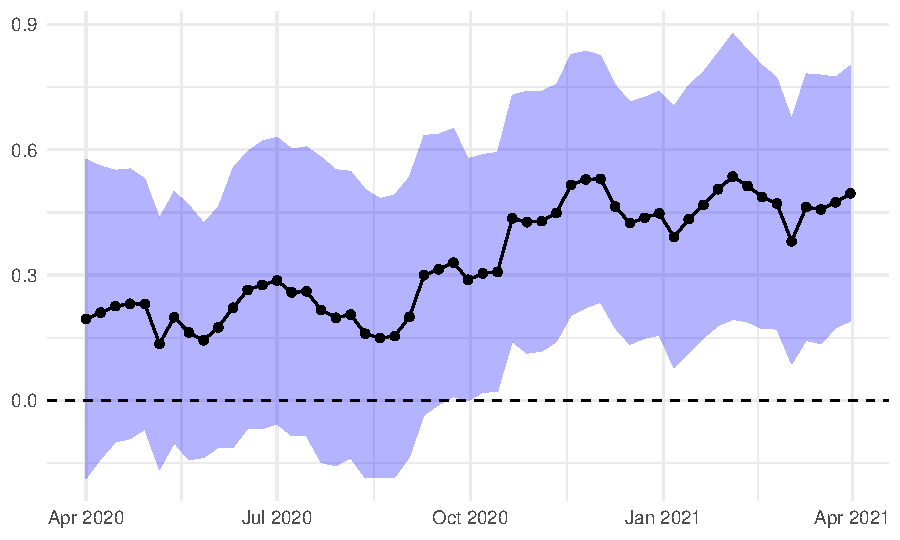
\includegraphics[width=0.8\linewidth]{write_up_test_files/figure-latex/over-time-1} \caption{Effect of Distrust on Government Stringency Over Time}\label{fig:over-time}
\end{figure}

\hypertarget{including-other-low-level-variables}{%
\subsection{Including other low-level variables}\label{including-other-low-level-variables}}

Table \ref{tab:addit} shows a table of models which include percentage change in transport and new deaths per million, comparing them to Model 9 which is the main model in this paper. A lagged version of both variables is used because the effect that either has on government stringency is likely to take time. For instance, when new deaths increase to a level where a government wants to increase the stringency of restrictions the process of introducing a new policy may take time. How many days of lag to use is calculated by creating multiple models with a lag from 1 to 50 days and using the days of lag for which there is the strongest association between the coefficient and government stringency. All of these models control for the same variables as in Model 9. Figure \ref{fig:lag-deaths} shows how increasing days of lag affects the association for new deaths per million and figure \ref{fig:lag-trans} shows how the association changes for change in transport use.~For both new deaths per million and change in transport use, 1 day of lag has the strongest association with government stringency, as such this is the level of lag used in the models in table \ref{tab:addit}\footnote{While the strongest association between change in transport use and government stringency occurs with one day of lag, the association is negative when it is expected to be positive. This potentially leads to a further misspecification of the model, hence why it is only done the additional analysis.}.\\
~\\
In model 10, when new deaths per million is included, the estimate of distrust remains similar to model 9 (0.31) and remains significant. When change in transport use is included in models 11 and 12, the estimate drops slightly and becomes insignificant, showing that change in transport use is potentially confounding the estimate\footnote{Although the estimate being insignificant may be the result of fewer countries being included in the model. A drop from 64 to 59.}. However, the direction of the coefficient on change in transport use indicates that this is a misspecification of the model. The coefficient in model 13 indicates that for a one unit increase in change in transport (which is substantively an increase in the number of people using transport) the stringency index decreases by 0.52 The coefficients on change in transport in model 11 and 12 shows the problem with including transport in the main model. In theory this coefficient should be positive, such that an increase in percentage change in transport (which in substantial terms would be more people using public transport) would result in the government imposing stricter restrictions. We do not see this in the model because there are long periods of time when both few people are using public transport and government restrictions are high. Therefore, the variables are not included in the main model but as the estimates of distrust remain similar there is still strong evidence in support of the hypothesis.\\

\hypertarget{other-policy-measures}{%
\subsection{Other policy measures}\label{other-policy-measures}}

Another additional analysis conducted is comparing models with difference policy response indices from the OxCGRT project, as the outcome variable. The main policy response used in this study is the stringency index, which is made up of the indicators on lockdown policies. Other indices include the containment and health index, which is the stringency index with the addition of indicators on testing and contact tracing. The economic support index is comprised of indicators which measure a government economic policy in response to the pandemic, such as income support and debt relief. Finally, the overall government response index is comprised of all indicators of government pandemic policy (Hale, et al., 2021). Table \ref{tab:policy} shows the results from these models, compared with model 9, which has the stringency index as the outcome.\\
~\\
The models show that with the containment and health index as the outcome variable the estimated effect of distrust remains similar (0.35) and also has a higher level of confidence (99.9\%). When the financial support index is the outcome variable, the estimated effect of distrust remains at a similar level (0.32) but with a large increase in the standard error (0.21) this result is not significant. The last model, which has the overall response index as the outcome variable, again shows a similar result to model 9 and with a higher level of confidence. This model is substantively less interesting, as it is not possible to tell exactly what the level of distrust is having an effect on, but it does add some further robustness in the support of the hypothesis.\\

\begin{table}
\caption{Models with different policy measures}
\begin{center}
\begin{small}
\begin{tabular}{l c c c c}
\hline
 & Stringency
Index & Containment
Index & Economic
Response & Overall
Response \\
\hline
Distrust in People        & $0.33^{**}$ & $0.35^{***}$ & $0.32$   & $0.34^{***}$ \\
                          & $(0.12)$    & $(0.09)$     & $(0.21)$ & $(0.09)$     \\
\hline
Num. obs.                 & $28479$     & $28428$      & $28451$  & $28427$      \\
Num. groups: location     & $64$        & $64$         & $64$     & $64$         \\
Var: location (Intercept) & $107.43$    & $72.26$      & $344.74$ & $69.51$      \\
Var: Residual             & $246.94$    & $151.56$     & $356.86$ & $138.37$     \\
\hline
\multicolumn{5}{l}{\tiny{$^{***}p<0.001$; $^{**}p<0.01$; $^{*}p<0.05$}}
\end{tabular}
\end{small}
\label{tab:policy}
\end{center}
\end{table}

\hypertarget{discussion}{%
\subsection{Discussion}\label{discussion}}

This paper has sought to test the the effect that distrust in people has on government stringency during the pandemic. These results show strong evidence that the hypothesis is true -- that higher levels of distrust in people causes higher levels of stringency -- with a significant positive estimate of distrust across all model specifications. This adds further support to the current literature on the important role that interpersonal trust has played during the Covid-19 pandemic. The result also supports the theory that trust plays an important role in solving collective action problems. However, the precise mechanism at play here has not been tested. The theory proposed in this paper suggests that higher distrust will lead to higher policy stringency due to increased demand for the government to intervene in solving the Covid-19 collective action problem. The results only show that higher trust leads to more government stringency, not that it leads to increased demand for stringency which then leads to more stringency. It is possible that some other mechanism is at play here, for example it might be that higher levels of distrust within the population leads to government officials also being distrusting and therefore do not trust people to take steps to reduce the spread of Covid-19 without intervention. It is also possible that a combination of mechanisms is at play. Further analysis beyond the scope of this paper is needed in order to test this, but the results of this study offer the initial evidence needed to fuel further research.\\
~\\
For example, a key piece of research needed to support the theory offered in this paper is to test if distrust leads to more demand and support for Covid-19 restrictions. Using cross-national survey data on support for school closures (YouGov Plc, 2020), a preliminary analysis is conducted using a simple bivariate regression, showing that there is a positive correlation between a countries level of distrust and support for Covid-19 restrictions, Figure /\ref{fig:yougov} shows this relationship. This is not a robust analysis, with only 16 countries in the sample, but does show that there is a possible relationship between distrust and support for restrictions which would further support the evidence of the mechanism proposed in this paper. But more research is needed to see if this relationship is robust and holds with more countries in the sample.\\
~\\

\begin{figure}
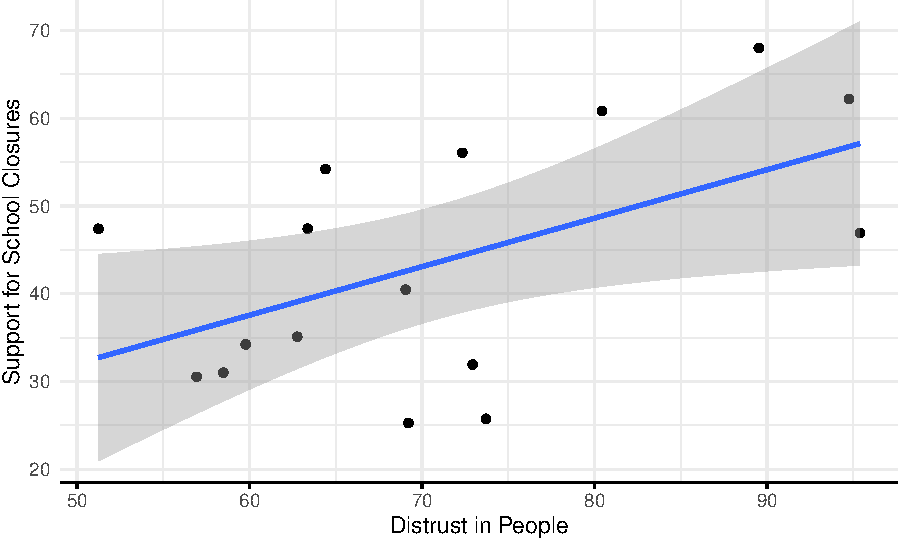
\includegraphics[width=0.8\linewidth]{write_up_test_files/figure-latex/yougov-1} \caption{Preliminary Analysis Showing the Relationship Between Distrust and Support for School Closures}\label{fig:yougov}
\end{figure}

\hfill\break
The results also show that the effect of distrust has increased as the pandemic went on, with no significant effect until October 2020 after which the effect remained significant throughout. The increase of the estimate of distrust during the autumn and winter might be explained due to this being a time when many countries began experiencing a second wave of Covid-19 cases. In the beginning of the pandemic in March 2020 many governments rushed to impose very strict restrictions as little was known about the virus and governments did not want to risk being overrun by it. But then in the second wave, many countries had increased opposition to lockdown restrictions and during this time other factors, including levels of distrust, were more likely to have an effect on government stringency. This might explain why the effect of distrust increased but further research, perhaps qualitative, would be needed to confirm the mechanism at play.\\
~\\
The final models in the results show that when government financial support is the outcome variable the estimate of distrust become insignificant. This result is not problematic for the theory proposed in this paper and it can fit within the causal mechanism of collective action. The level of distrust is unlikely to change the demand for economic intervention from the government. This is because it is in the individual interest of most individuals to receive financial support from the government independent of how distrusting they are of others.\\

\hypertarget{limitations-and-assumptions}{%
\section{Limitations and Assumptions}\label{limitations-and-assumptions}}

\hypertarget{selection-bias}{%
\subsection{Selection bias}\label{selection-bias}}

The main limitation of this study is potentially remaining selection bias. As the level of distrust is not randomly assigned to countries there may be an uncontrolled for factor that leads to some countries having higher levels of distrust which is also associated with having higher levels of stringency, as a result it may not be distrust that has a causal effect on stringency but some other variable that has not been included. Although many potentially confounding variables have been adjusted for, including measures of economic, cultural and political factors, there may be remaining confounding variables that have not been adjusted for. This potentially confounding variable that has not been adjusted for is likely to be some unquantified cultural or political factor, for instance, a major cultural event (such as large terrorist attack or financial crisis) can have a significant effect on levels of distrust and also change the way governments responds to crises.\\
~\\
These cultural shocks should be controlled for with the inclusion of the conflict index, which does quantify events such as terrorist attacks and government crises. But only the 2019 conflict index is included, so any cultural shocks from 2018 and before will not be adjusted for in the models. This is limiting because evidence has shown that the effect of these cultural shocks can, in some cases, continue for years after the event (Giordano \& Lindstrom, 2016). However, these major culture changing shocks are relatively rare and should not affect many of the countries in this study and therefore should not have a large effect on the estimate of the effect of distrust. It is important to keep in mind though, that the results of the analysis do assume that all potentially confounding factors are adjusted for and if this assumption does not hold, then the estimate of distrust may be unreliable.\\

\hypertarget{number-of-countries}{%
\subsection{Number of Countries}\label{number-of-countries}}

There are some potential problems with the number of countries used in the analysis. As more variables are added to the models in Table 2 the number of countries in the model reduces. In the bivaraite models with only distrust and government stringency included there are 72 countries, but this reduces to 64 countries for model 9. This begs the question of whether the change in estimate from model 2 to model 9 is due to having adjusted for confounders or because of the removal of countries from the model. Table \ref{tab:obs-test} shows that even if model 2 had only the 64 countries included in model 9 the estimate of distrust would be the same (shown in model 2B). This supports the robustness of the results in model 9, showing that it is due to having adjusted for confounders and not due to having a different group of countries in the model.\\

\begin{figure}
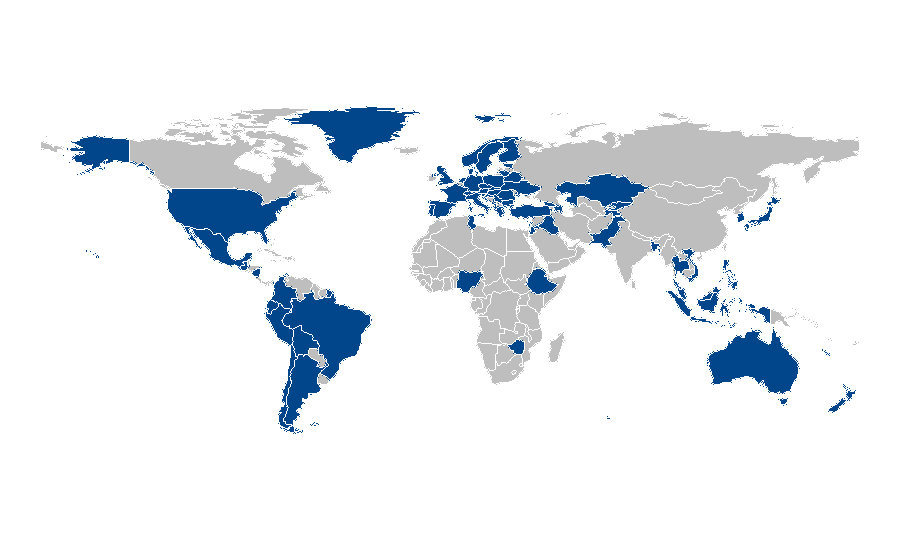
\includegraphics[width=0.8\linewidth]{write_up_test_files/figure-latex/map-1} \caption{Map of Countries Included in Model 9}\label{fig:map}
\end{figure}

A second limitation of the number of countries used is the generalisability of the results. There are relatively few countries for which there is data on the level of distrust, which is why there are only 72 countries used in the bivariate model and this number drops to 64 because of the lack of data available for other variables. These 64 countries, highlighted on a map in Figure \ref{fig:map}, are not representative of the world as a whole. The countries in the sample are mostly from Europe, the Americas and a few countries from South East Asia. Most notably there are only a small number of African countries included. The countries that are not included tend to be those that have lower economic development, which means that when interpreting the results of this study they cannot be applied with certainty to less developed countries. It is only possible to say that for the sample included in the main model, higher levels of distrust lead to higher levels of stringency in response to the pandemic.\\

\hypertarget{statistical-assumptions}{%
\subsection{Statistical Assumptions}\label{statistical-assumptions}}

There are a few statistical assumptions that a random effects model makes. Graphs that attempt to test whether these assumptions are met are in the Appendix and all the graphs are calculated based off model 9. Figure \ref{fig:homo} shows the homogeneity of residuals\footnote{Residuals are standardised and calculated using the empirical Bayes method.} (Loy \& Hofmann, 2014). There appears to be clusters of residuals, but these will be the residuals for each country, and other than that there does not appear to be problems with the homogeneity of residuals. Figure \ref{fig:vif} shows the variance inflation factors (VIF) for the main model (Fox \& Weisberg, 2019). Other than some moderate correlation with logged GDP and education index, all have a low VIF, and the estimate of distrust is not likely to be affected. Figure \ref{fig:dfbetas} shows the DFBETAS for the coefficient on distrust, this is a measure of how much the estimate of distrust is changed when removing each country from the model (Nieuwenhuis, et al., 2012). Although some countries have a large influence on the estimate, such as New Zealand and Ukraine, removing any country from the model does not change the direction of the estimate of distrust or whether it is significant. Overall, these statistical tests do not pose problems for the results of this study.\\

\hypertarget{conclusion}{%
\section{Conclusion}\label{conclusion}}

The Covid-19 pandemic is one of the most significant recent collective action problems that the world has faced. With the virus causing a staggering number of deaths and hospitalisations, governments around the world have had to act quickly in response to pandemic and impose lockdown style restrictions. It was expected that countries having higher levels of distrust in others would result in higher levels of stringency and the analysis in this provides strong support for this. By using a random effects regression analysis, the effect of distrust on government stringency was estimated, with the results showing a significant positive effect. This empirical finding provides strong support for the hypothesis and, alongside the other literature, shows the important role that interpersonal trust has had on Covid-19 outcomes during the pandemic.\\
~\\
The other key finding of the study shows that the effect of distrust increased as the pandemic went on. The effect of distrust is estimated over time by splitting the pandemic into seven-day periods and conducting the same random effects analysis, showing that in October 2020, the effect began to increase and then was steady going into the new year. It is proposed that this is due to most governments having a very stringent initial response to the pandemic but then other political and societal factors -- such as distrust -- were able to play more of a role once the second wave began.\\
~\\
These results rest upon the assumption that all confounding factors have been adjusted for and great effort has been made to ensure that this is the case, but it is still possible that a confounder has been omitted that would change the estimate of distrust and any interpretation of the results should keep this in mind. The generalisability of the analysis is also important when interpreting the results. With only 64 countries included in the main model the results can only be applied with certainty to those countries and cannot be extrapolated to countries outside the sample.\\
~\\
The results provide support for treating the pandemic as a collective action problem and for the role that interpersonal trust plays in solving collective action problems. They also provide initial support for the theoretical mechanism proposed, that higher levels of distrust create a demand for higher stringency which is then fulfilled by the government (although further research is needed to confirm the precise mechanism). With the pandemic likely to be far from over, the effect that distrust has on government stringency may still change and future research should reconsider its effect as well as the effect it has on other parts of government response. In particular this paper has not considered the effect that distrust has on vaccine policy, which is playing an increasing role in the more recent part of the pandemic. Understanding the factors that affect how the pandemic, as a collective action problem, has been solved will be important in knowing how to approach other large-scale collective action problems facing the world, such as climate change.\\

\newpage

\hypertarget{references}{%
\section*{References}\label{references}}
\addcontentsline{toc}{section}{References}

Banks, A. S. \& Wilson, K. A., 2020. Cross-National Time-Series Data Archive (CNTS), Jerusalem: Databanks International.\\
Bargaina, O. \& Aminjonov, U., 2020. Trust and compliance to public health policies in times of COVID-19. Journal of Public Economics, Volume 192.\\
Bates, D., Maechler, M., Bolker, B. \& Walker, S., 2015. Fitting Linear Mixed-Effects Models Using lme4. Journal of Statistical Software, 67(1), pp.~1-48.\\
Bell, A. \& Jones, K., 2015. Explaining Fixed Effects: Random Effects Modeling of Time-Series Cross-Sectional and Panel Data. Political Science Research and Methods, 3(1), pp.~133-153.\\
Bhadra, A., Mukherjee, A. \& Sarkar, K., 2021. Impact of population density on Covid-19 infected and mortality rate in India. Modeling Earth Systems and Environment, Volume 7, pp.~623-629.\\
Bjornskov, C., 2012. How Does Social Trust Affect Economic Growth?. Southern Economic Journal, 78(4), pp.~1346-1368.\\
Cucinotta, D. \& Vanelli, M., 2020. WHO Declares COVID-19 a Pandemic. Acta Biomed, 91(1), pp.~157-160.\\
Cucinotta, D. \& Vanelli, M., 2020. WHO Declares COVID-19 a Pandemic. Acta Biomed, 91(1), pp.~157-160.\\
Daniele, G. \& Geys, B., 2015. Interpersonal trust and welfare state support. European Journal of Political Economy, Volume 39, pp.~1-12.\\
Dong, E., Du, H. \& Gardner, L., 2020. An interactive web-based dashboard to track COVID-19 in real time. Lancet Infectious Diseases, 20(5), pp.~533-534.\\
Elgara, F. J., Stefaniakb, A. \& Wohl, M. J., 2020. The trouble with trust: Time-series analysis of social capital, income inequality, and COVID-19 deaths in 84 countries. Social Science \& Medicine, Volume 263.\\
EVS/WVS, 2021a. European Values Study and World Values Survey: Joint EVS/WVS 2017-2021 Dataset, s.l.: JD Systems Institute \& WVSA.\\
EVS/WVS, 2021b. European Values Study and World Values Survey: Joint EVS/WVS 2017-2021 Dataset - Variable Report (Documentation/Tables). s.l.:GESIS Data Archive, Cologne and JD Systems Institute.\\
Fox, J. \& Weisberg, S., 2019. An R Companion to Applied Regression. 3rd Edition ed.~Thousand Oaks: Sage.\\
Giordano, G. N. \& Lindstrom, M., 2016. The 2005 London terror attacks: An investigation of changes in psychological wellbeing and social capital pre- and post-attacks (2003-07)-A UK panel study. SSM - Population Health, Volume 2, pp.~485-494.\\
GlobeNewswire, 2020. Coronavirus (COVID-19): Global Market Conditions, Vaccines, Trials and Potential Treatments. {[}Online{]}\\
Available at: \url{https://advance.lexis.com/api/permalink/ae7c2029-a2d4-4750-8f85-a70a6f7330f8/?context=1519360\&federationidp=CZVRR460015} {[}Accessed August 2021{]}.\\
Goldstein, D. A. N. \& Wiedemann, J., 2021. Who Do You Trust? The Consequences of Partisanship and Trust for Public Responsiveness to COVID-19 Orders. Perspectives on Politics, pp.~1-27.\\
Google LLC, 2021. Google COVID-19 Community Mobility Reports. {[}Online{]}\\
Available at: \url{https://www.google.com/covid19/mobility/} {[}Accessed May 2020{]}.\\
Guiso, L., Sapienza, P. \& Zingales, L., 2004. The role of social capital in financial development. American Economic Review, 94(3), pp.~526-556.\\
Guiso, L., Sapienza, P. \& Zingales, L., 2009. Cultural biases in economic exchange?. The Quarterly Journal of Economics, 124(3), pp.~1095-1131.\\
Häuberer, J., 2011. The Founding Concepts of Social Capital - Bourdieu's Theory of Capital and Coleman's Rational-Choice Approach to Social Capital. In: Social Capital Theory. s.l.:VS Verlag für Sozialwissenschaften.\\
Hale, T. et al., 2021. A global panel database of pandemic policies (Oxford COVID-19 Government Response Tracker). Nature Human Behaviour, Volume 5, pp.~529-538.\\
Harring, N., Jagers, S. C. \& Lofgren, A., 2021. COVID-19: Large-scale collective action, government intervention, and the importance of trust. World Development, Volume 138.\\
Helliwell, J. F. \& Putnam, R. D., 1995. Economic Growth and Social Capital in Italy. Eastern Economic Journal , 21(3), pp.~295-307.\\
House, J. S. \& Wolf, S., 1978. Effects of urban residence on interpersonal trust and helping behavior. Journal of Personality and Social Psychology, 36(9), pp.~1029-1043.\\
Imai, K. \& Kim, I. S., 2019. When Should We Use Unit Fixed Effects Regression Models for Causal Inference with Longitudinal Data?. American Journal of Political Science, 63(2), pp.~467-490.\\
Knack, S., 2002. Social Capital and the Quality of Government: Evidence from the States. American Journal of Political Science, 46(4), pp.~772-785.\\
Lindström, M., 2020. A commentary on ``The trouble with trust: Time-series analysis of social capital, income inequality, and COVID-19 deaths in 84 countries''. Social Science \& Medicine, Volume 263.\\
Loy, A. \& Hofmann, H., 2014. HLMdiag: A Suite of Diagnostics for Hierarchical Linear Models in R. Journal of Statistical Software, 56(5), pp.~1-28.\\
Marshall, M. G. \& Gurr, T. R., 2020. Polity5 - Political Regime Characteristics and Transitions, 1800-2018 - Dataset Users' Manual. {[}Online{]}\\
Available at: \url{http://www.systemicpeace.org/inscr/p5manualv2018.pdf}\\
{[}Accessed August 2021{]}.\\
Nieuwenhuis, R., Grotenhuis, M. t. \& Pelzer, B., 2012. influence.ME: Tools for Detecting Influential Data in Mixed Effects Models. R Journal, 4(2), pp.~38-47.\\
Nuclear Threat Initiative, Johns Hopkins Center for Health Security, The Economist Intelligence Unit, 2019. 2019 Global Health Security Index. {[}Online{]}\\
Available at: \url{https://www.ghsindex.org/}\\
{[}Accessed May 2021{]}.\\
Olson, M., 1965. The Logic of Collective Action: Public Goods and the Theory of Groups. Cambridge, Massachusetts: Harvard University Press.\\
Olson, M., 1982. The Logic. In: The Rise and Decline of Nations: Economic Growth, Stagnation, and Social Rigidities. s.l.:Yale University Press, pp.~17-32.\\
Ostrom, E., 2009. Collective Action Theory. In: C. Boix \& S. C. Stokes, eds.~The Oxford Handbook of Comparative Politics . Oxford: Oxford University Press.\\
R Core Team, 2020. R: A language and environment for statistical computing, Vienna: R Foundation for Statistical Computing.\\
Ritchie, H. et al., 2020a. Coronavirus (COVID-19) Deaths. {[}Online{]}\\
Available at: \url{https://ourworldindata.org/covid-deaths} {[}Accessed August 2020{]}.\\
Ritchie, H. et al., 2020b. COVID-19: Google Mobility Trends. {[}Online{]} Available at: \url{https://ourworldindata.org/covid-google-mobility-trends} {[}Accessed May 2021{]}.\\
Solt, F., 2020. Measuring Income Inequality Across Countries and Over Time: The Standardized World Income Inequality Database. Social Science Quarterly, 101(3), pp.~1183-1199.\\
Twenge, J. M., Campbell, W. K. \& Carter, N. T., 2014. Declines in Trust in Others and Confidence in Institutions Among American Adults and Late Adolescents. Psychological Science, 25(10), pp.~1914-1923.\\
United Nations Development Programme, 2020. Education index. {[}Online{]}\\
Available at: \url{http://hdr.undp.org/en/indicators/103706} {[}Accessed June 2021{]}.\\
Warren, M. E., 1999. Introduction. In: M. E. Warren, ed.~Democracy and Trust. Cambridge: Cambridge University Press, pp.~1-21.\\
World Bank, 2021a. GDP Growth (annual \%). {[}Online{]}\\
Available at: \url{https://data.worldbank.org/indicator/NY.GDP.MKTP.KD.ZG} {[}Accessed June 2021{]}.\\
World Bank, 2021b. GDP (current US\$). {[}Online{]}\\
Available at: \url{https://data.worldbank.org/indicator/NY.GDP.MKTP.CD} {[}Accessed May 2021{]}.\\
YouGov Plc, 2020. COVID-19: Level of support for actions governments could take. {[}Online{]}\\
Available at: \url{https://yougov.co.uk/topics/international/articles-reports/2020/03/17/level-support-actions-governments-could-take} {[}Accessed August 2021{]}.\\
Zak, P. J. \& Knack, S., 2001. Trust and Growth. The Economic Journal, Volume 111, pp.~195-321.\\

\newpage

\hypertarget{appendix}{%
\section*{Appendix}\label{appendix}}
\addcontentsline{toc}{section}{Appendix}

\setcounter{table}{0}  \renewcommand{\thetable}{A\arabic{table}} \setcounter{figure}{0} \renewcommand{\thefigure}{A\arabic{figure}}

\begin{figure}
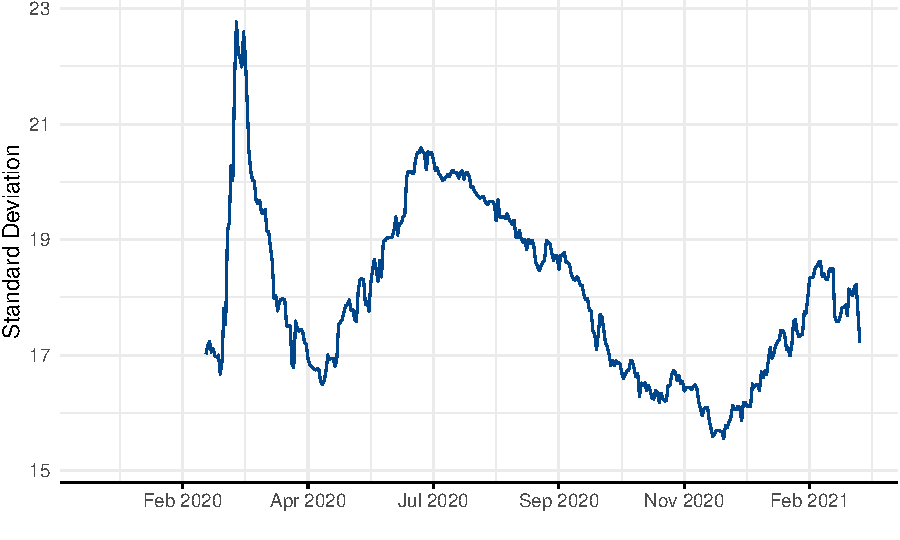
\includegraphics[width=0.8\linewidth]{write_up_test_files/figure-latex/stringency-sd-1} \caption{Standard Deviation of Government Stringency During the Pandemic}\label{fig:stringency-sd}
\end{figure}

\begin{figure}
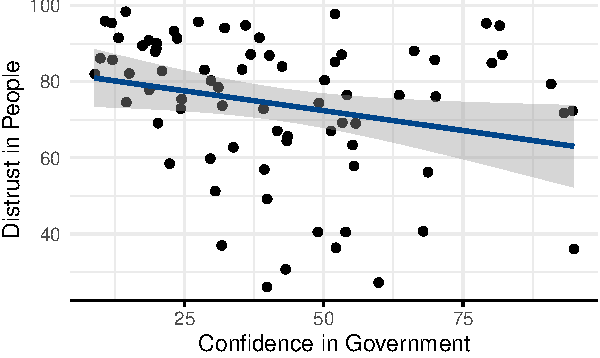
\includegraphics[width=0.48\linewidth]{write_up_test_files/figure-latex/conf-plots-1} 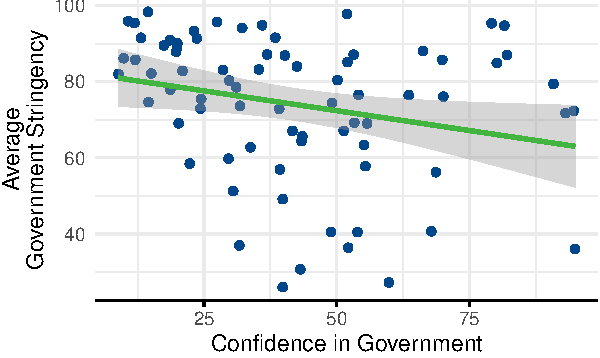
\includegraphics[width=0.48\linewidth]{write_up_test_files/figure-latex/conf-plots-2} \caption{Association of Confidence in Government with Distrust in People and Government Stringency}\label{fig:conf-plots}
\end{figure}

\begin{figure}
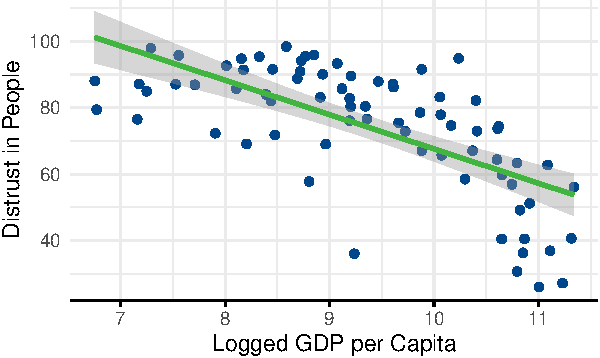
\includegraphics[width=0.48\linewidth]{write_up_test_files/figure-latex/gdp-plots-1} 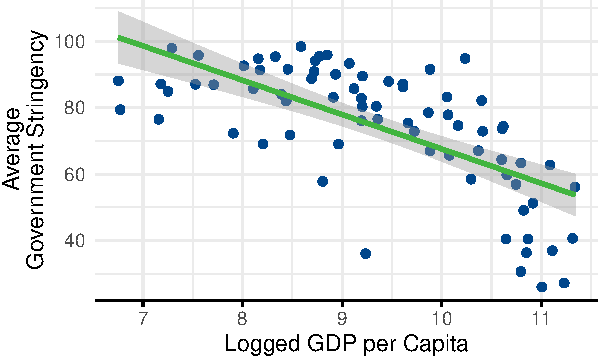
\includegraphics[width=0.48\linewidth]{write_up_test_files/figure-latex/gdp-plots-2} \caption{Association of Logged GDP per Capita with Distrust in People and Government Stringency}\label{fig:gdp-plots}
\end{figure}

\begin{figure}
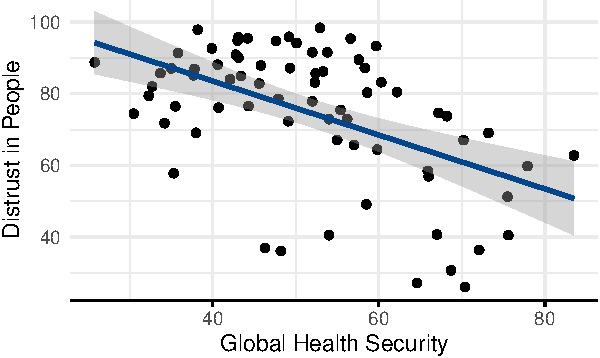
\includegraphics[width=0.48\linewidth]{write_up_test_files/figure-latex/ghs-plots-1} 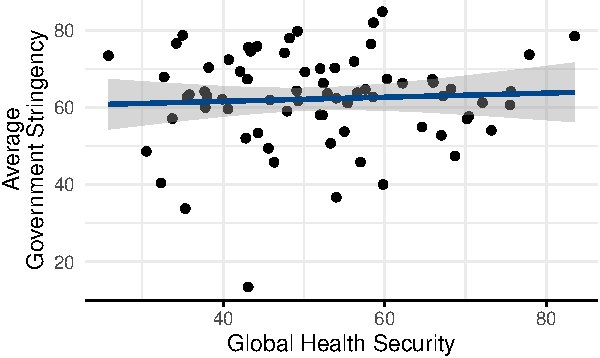
\includegraphics[width=0.48\linewidth]{write_up_test_files/figure-latex/ghs-plots-2} \caption{Association of GHS with Distrust in People and Government Stringency}\label{fig:ghs-plots}
\end{figure}

\begin{figure}
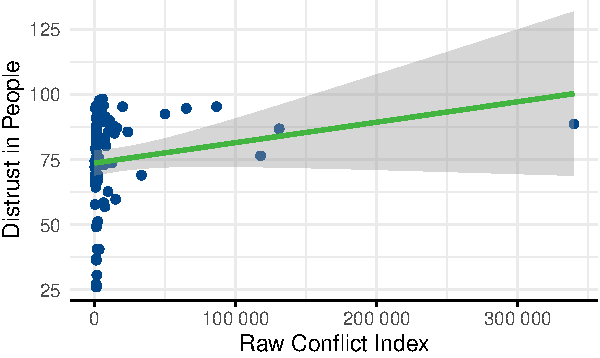
\includegraphics[width=0.48\linewidth]{write_up_test_files/figure-latex/conflict-log-1} 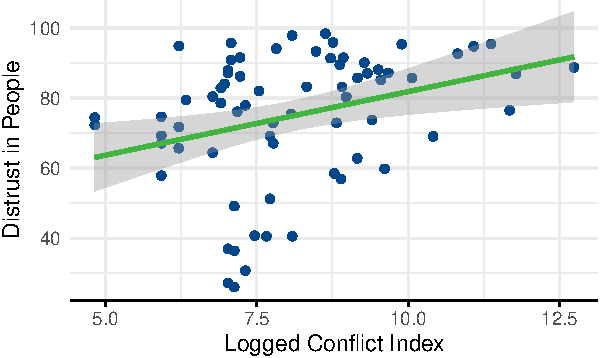
\includegraphics[width=0.48\linewidth]{write_up_test_files/figure-latex/conflict-log-2} \caption{Raw vs. Logged Conflict Index Relationship with Distrust in People}\label{fig:conflict-log}
\end{figure}

\begin{figure}
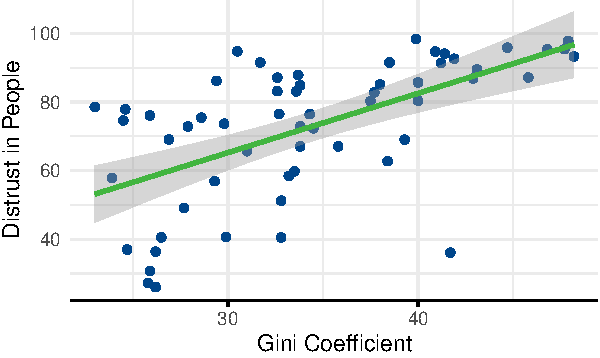
\includegraphics[width=0.48\linewidth]{write_up_test_files/figure-latex/gini-plots-1} 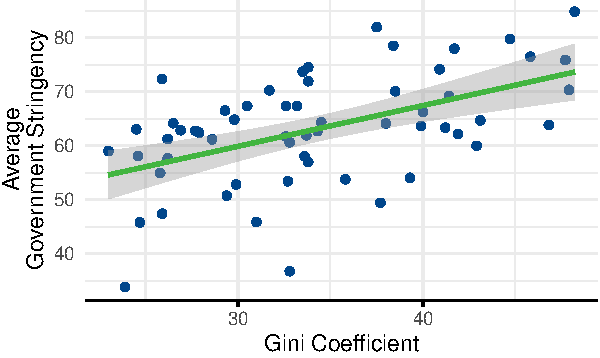
\includegraphics[width=0.48\linewidth]{write_up_test_files/figure-latex/gini-plots-2} \caption{Association of Gini Coefficient with Distrust in People and Government Stringency}\label{fig:gini-plots}
\end{figure}

\begin{figure}
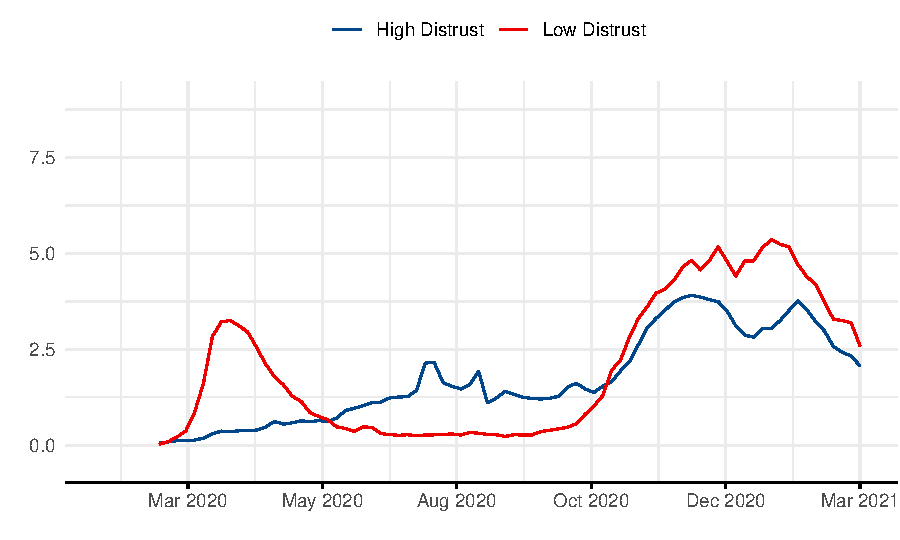
\includegraphics[width=0.8\linewidth]{write_up_test_files/figure-latex/deaths-change-1} \caption{Average Daily Covid-19 deaths per Million during the pandemic}\label{fig:deaths-change}
\end{figure}

\begin{figure}
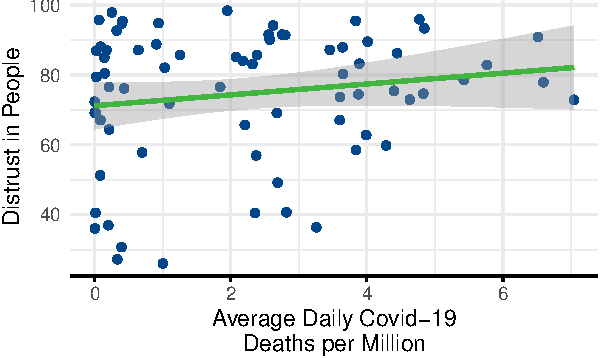
\includegraphics[width=0.48\linewidth]{write_up_test_files/figure-latex/deaths-plots-1} 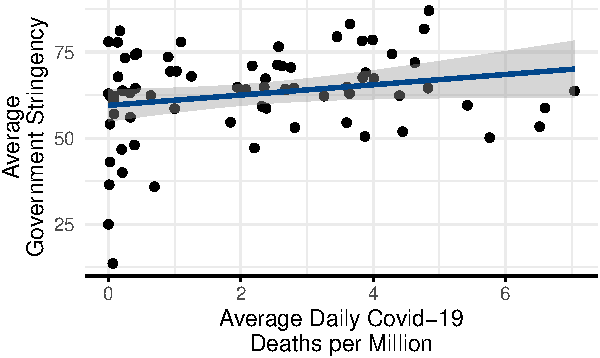
\includegraphics[width=0.48\linewidth]{write_up_test_files/figure-latex/deaths-plots-2} \caption{Association of Average Daily Covid-19 Deaths per Million with Distrust in People and Government Stringency}\label{fig:deaths-plots}
\end{figure}

\begin{figure}
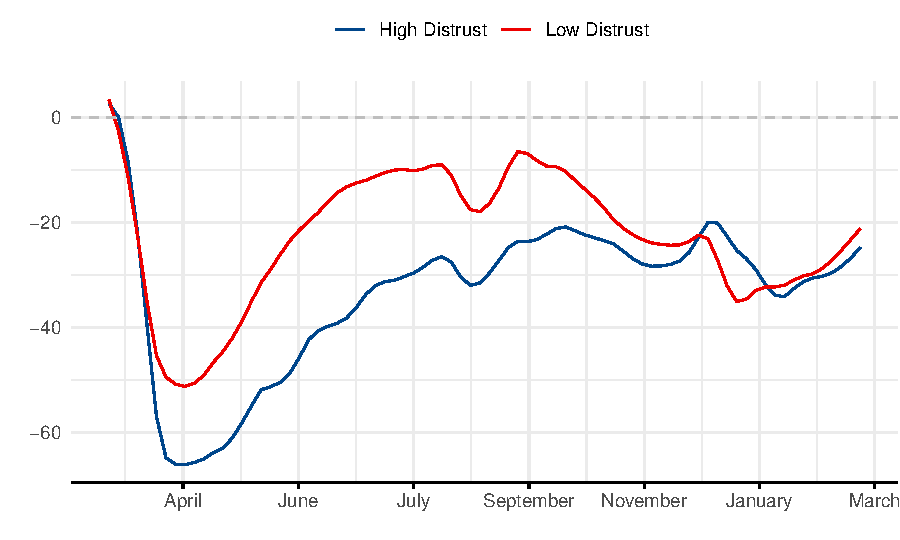
\includegraphics[width=0.8\linewidth]{write_up_test_files/figure-latex/mobility-plot-1} \caption{Change in use of Public Transport during the Covid-19 pandemic}\label{fig:mobility-plot}
\end{figure}

\begin{figure}
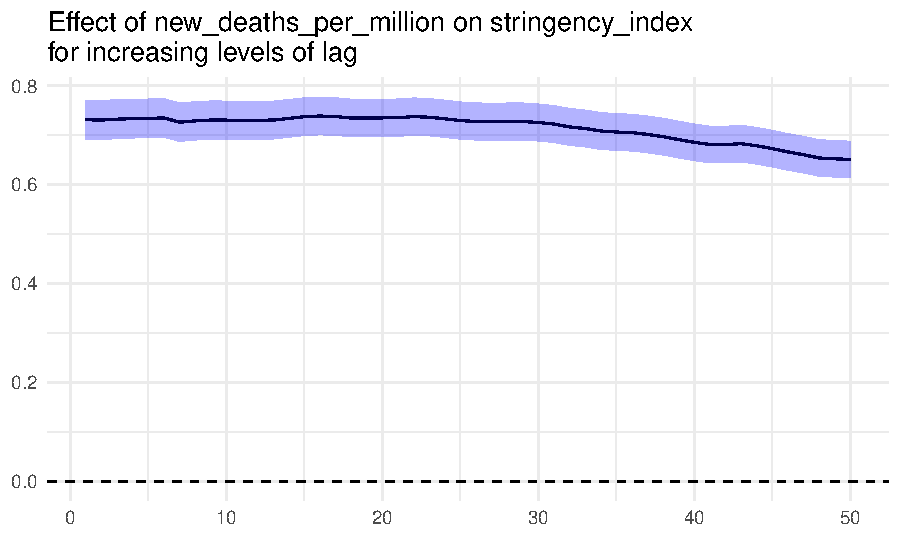
\includegraphics[width=0.8\linewidth]{write_up_test_files/figure-latex/lag-deaths-1} \caption{The Coefficient on New deaths per Million for increasing days of lag}\label{fig:lag-deaths}
\end{figure}

\begin{figure}
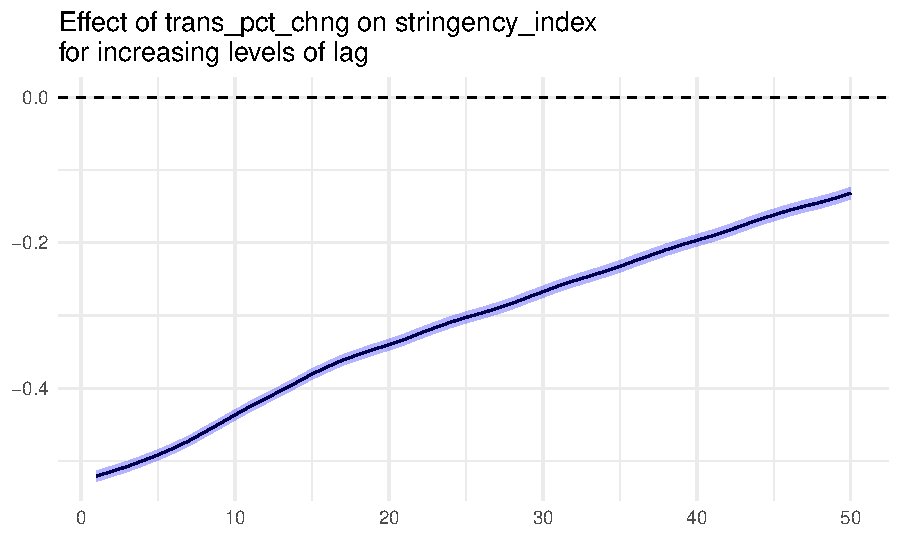
\includegraphics[width=0.8\linewidth]{write_up_test_files/figure-latex/lag-trans-1} \caption{The Coefficient on Change in Transport for increasing days of lag}\label{fig:lag-trans}
\end{figure}

\begin{table}
\caption{Models Including Daily Deaths and Percent Change in Transport}
\begin{center}
\begin{small}
\begin{tabular}{l c c c c c}
\hline
 & Model 9 & Model 12 & Model 13 & Model 14 & Model 15 \\
\hline
Distrust in People                & $0.33^{**}$  & $0.31^{**}$  & $0.27$        & $0.26$        & $0.01^{*}$    \\
                                  & $(0.12)$     & $(0.11)$     & $(0.14)$      & $(0.13)$      & $(0.00)$      \\
Log of GDP per Capita             & $6.00^{*}$   & $5.90^{*}$   & $4.34$        & $4.13$        & $0.11$        \\
                                  & $(2.95)$     & $(2.91)$     & $(3.62)$      & $(3.53)$      & $(0.10)$      \\
GDP Growth                        & $0.59$       & $0.53$       & $0.95$        & $0.86$        & $0.02$        \\
                                  & $(0.52)$     & $(0.51)$     & $(0.59)$      & $(0.58)$      & $(0.02)$      \\
Education Index                   & $28.17$      & $27.17$      & $22.87$       & $25.78$       & $0.80$        \\
                                  & $(22.37)$    & $(22.05)$    & $(27.99)$     & $(27.33)$     & $(0.75)$      \\
Population over age 65            & $-1.06^{**}$ & $-1.17^{**}$ & $-0.51$       & $-0.64$       & $-0.02$       \\
                                  & $(0.39)$     & $(0.38)$     & $(0.44)$      & $(0.43)$      & $(0.01)$      \\
Global Health Security Index      & $0.11$       & $0.10$       & $0.00$        & $0.01$        & $0.00$        \\
                                  & $(0.17)$     & $(0.16)$     & $(0.20)$      & $(0.20)$      & $(0.01)$      \\
Polity                            & $-0.38$      & $-0.40$      & $-0.47$       & $-0.46$       & $-0.02$       \\
                                  & $(0.39)$     & $(0.38)$     & $(0.44)$      & $(0.43)$      & $(0.01)$      \\
Log of Conflict Index             & $2.39^{*}$   & $2.39^{*}$   & $2.75^{*}$    & $2.79^{*}$    & $0.09^{**}$   \\
                                  & $(1.06)$     & $(1.04)$     & $(1.19)$      & $(1.16)$      & $(0.03)$      \\
Population Density                & $0.01$       & $0.01$       & $0.01$        & $0.01$        & $0.00^{*}$    \\
                                  & $(0.01)$     & $(0.01)$     & $(0.01)$      & $(0.01)$      & $(0.00)$      \\
Confidence in Government          & $-0.07$      & $-0.05$      & $-0.06$       & $-0.06$       & $-0.00$       \\
                                  & $(0.09)$     & $(0.09)$     & $(0.11)$      & $(0.11)$      & $(0.00)$      \\
New Deaths per Million lag 1      &              & $0.73^{***}$ &               & $0.39^{***}$  & $0.02^{***}$  \\
                                  &              & $(0.02)$     &               & $(0.02)$      & $(0.00)$      \\
Percent Change in Transport lag 1 &              &              & $-0.52^{***}$ & $-0.45^{***}$ & $-0.01^{***}$ \\
                                  &              &              & $(0.00)$      & $(0.00)$      & $(0.00)$      \\
Stringency Index lag 1            &              &              &               &               & $0.97^{***}$  \\
                                  &              &              &               &               & $(0.00)$      \\
\hline
Num. obs.                         & $28479$      & $27280$      & $26046$       & $25007$       & $25006$       \\
Num. groups: location             & $64$         & $64$         & $59$          & $59$          & $59$          \\
Var: location (Intercept)         & $107.43$     & $104.40$     & $127.73$      & $121.76$      & $0.08$        \\
Var: Residual                     & $246.94$     & $181.54$     & $134.16$      & $104.09$      & $5.18$        \\
\hline
\multicolumn{6}{l}{\tiny{$^{***}p<0.001$; $^{**}p<0.01$; $^{*}p<0.05$}}
\end{tabular}
\end{small}
\label{tab:addit}
\end{center}
\end{table}

\begin{table}
\caption{Models Testing the Effect of Removing Countries from the Bivariate Model}
\begin{center}
\begin{small}
\begin{tabular}{l c c c}
\hline
 & Model 2 & Model 2B & Model 9 \\
\hline
Distrust in People           & $0.20^{*}$ & $0.20^{*}$ & $0.33^{**}$  \\
                             & $(0.08)$   & $(0.08)$   & $(0.12)$     \\
Log of GDP per Capita        &            &            & $6.00^{*}$   \\
                             &            &            & $(2.95)$     \\
GDP Growth                   &            &            & $0.59$       \\
                             &            &            & $(0.52)$     \\
Education Index              &            &            & $28.17$      \\
                             &            &            & $(22.37)$    \\
Population over age 65       &            &            & $-1.06^{**}$ \\
                             &            &            & $(0.39)$     \\
Global Health Security Index &            &            & $0.11$       \\
                             &            &            & $(0.17)$     \\
Polity                       &            &            & $-0.38$      \\
                             &            &            & $(0.39)$     \\
Log of Conflict Index        &            &            & $2.39^{*}$   \\
                             &            &            & $(1.06)$     \\
Population Density           &            &            & $0.01$       \\
                             &            &            & $(0.01)$     \\
Confidence in Government     &            &            & $-0.07$      \\
                             &            &            & $(0.09)$     \\
\hline
Random Effects               & Yes        & Yes        & Yes          \\
Num. obs.                    & $33819$    & $28479$    & $28479$      \\
Num. groups: location        & $76$       & $64$       & $64$         \\
Var: location (Intercept)    & $164.46$   & $139.40$   & $107.43$     \\
Var: Residual                & $232.19$   & $246.94$   & $246.94$     \\
\hline
\multicolumn{4}{l}{\tiny{$^{***}p<0.001$; $^{**}p<0.01$; $^{*}p<0.05$}}
\end{tabular}
\end{small}
\label{tab:obs-test}
\end{center}
\end{table}

\begin{figure}
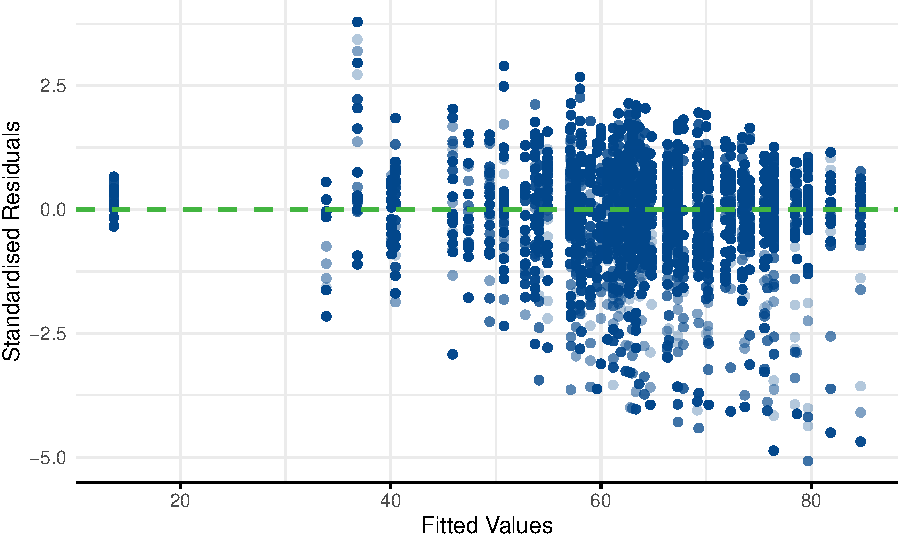
\includegraphics[width=0.8\linewidth]{write_up_test_files/figure-latex/homo-1} \caption{Homogeneity of Residuals}\label{fig:homo}
\end{figure}

\begin{figure}
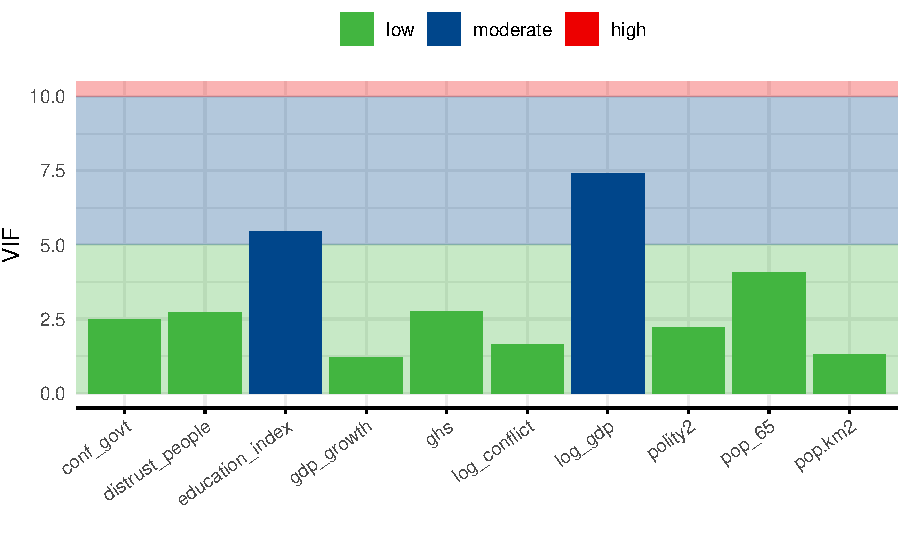
\includegraphics[width=0.8\linewidth]{write_up_test_files/figure-latex/vif-1} \caption{Variance Inflation Factors}\label{fig:vif}
\end{figure}

\begin{figure}
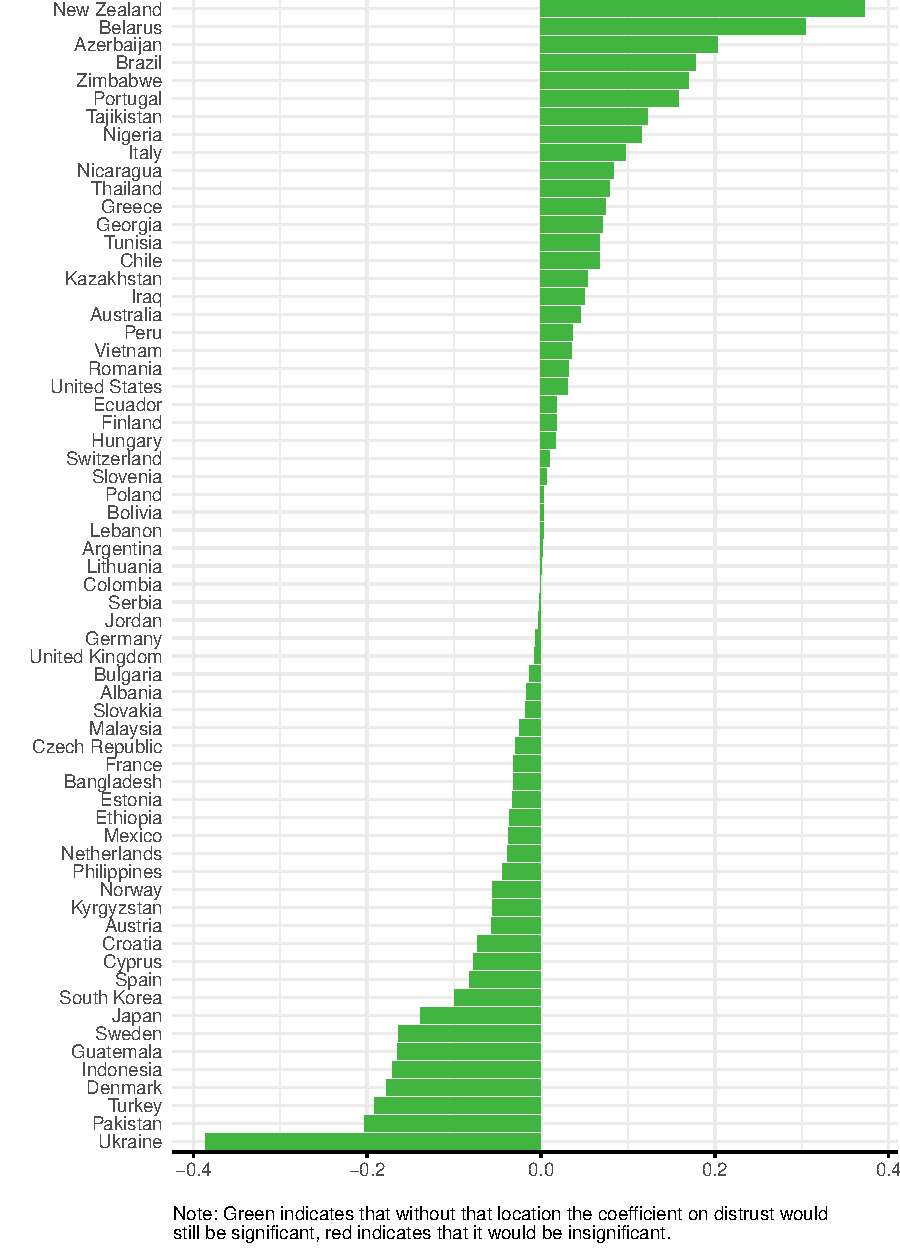
\includegraphics[width=0.8\linewidth]{write_up_test_files/figure-latex/dfbetas-1} \caption{DFBETAS}\label{fig:dfbetas}
\end{figure}

\end{document}
